\documentclass[dvipdfmx]{article}
\usepackage[dvipdfmx]{graphicx}
\usepackage{amsmath, amssymb}
\usepackage{mathtools}
\usepackage{here}
\begin{document}
\title{Weekly Report}
\author{Riku Gondow}
\maketitle
\section{Progress}
\begin{itemize}
    \item Consider how to evaluate the dataset
    \begin{itemize}
        \item Run the Baseline method code again, and average the accuracy
    \end{itemize}
    \item Read and Understand a paper to improve Loss function of Baseline
    \item Implement Triple Joint Loss\cite{tripleloss}
\end{itemize}

\section{Results of Baseline}
\begin{figure}[H]
\begin{center}
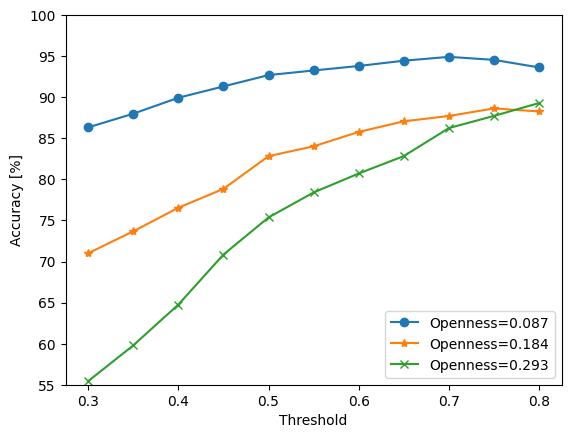
\includegraphics[width=0.8\linewidth]{./img/openset_graph.png}
\end{center}
\caption{Result (n=1)}
\end{figure}

\begin{figure}[H]
\begin{center}
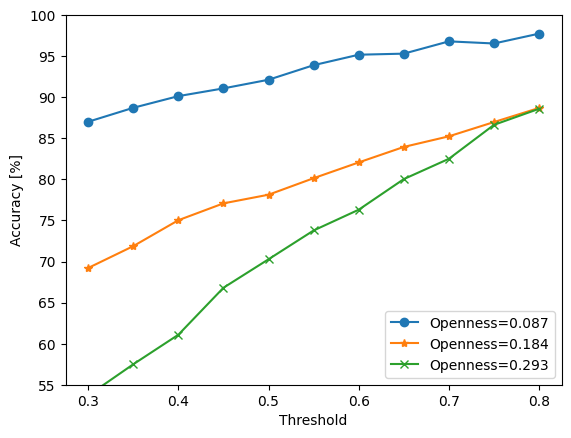
\includegraphics[width=0.8\linewidth]{./img/openset_graph2.png}
\end{center}
\caption{Result (n=5)}
\end{figure}

\begin{figure}[H]
\begin{center}
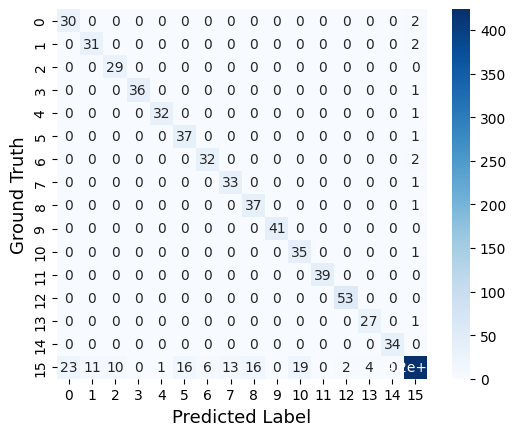
\includegraphics[width=0.8\linewidth]{./img/conf_threshold_1104.png}
\end{center}
\caption{Confusion Matrix (openness=0.293, threshold=0.8)}
\end{figure}


\begin{thebibliography}{99}
\bibitem{tripleloss} Y. Yang, B. Huang and Z. Ni, "Open-set Person Identification with Triple-Joint Loss Based on Radar Gait Micro-Doppler Signatures," 2022 7th International Conference on Intelligent Computing and Signal Processing (ICSP), 2022, pp. 1787-1791
\end{thebibliography}
\end{document}